\section{Approach}
\label{sec:approach}

The overall structure of this section can follow my previous work~\cite{chen2017unsupervised}.

\subsection{Finding similar technique}

We find similar technique within Stack Overflow tags based on word embedding and categorical information.

\subsubsection{Learning Tag Embeddings}
\label{sec:w2v}

\begin{figure}
	\centering
	\subfigure[Continuous skip-gram model]{%
		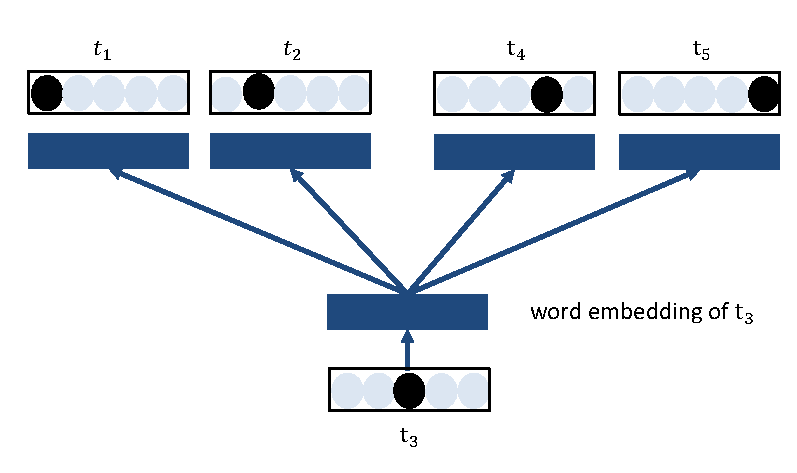
\includegraphics[width=0.23\textwidth]{figures/w2v_skip.pdf}
		\label{fig:w2v_skip}
	}
	\hfill
	\subfigure[Continuous bag-of-words model]{%
		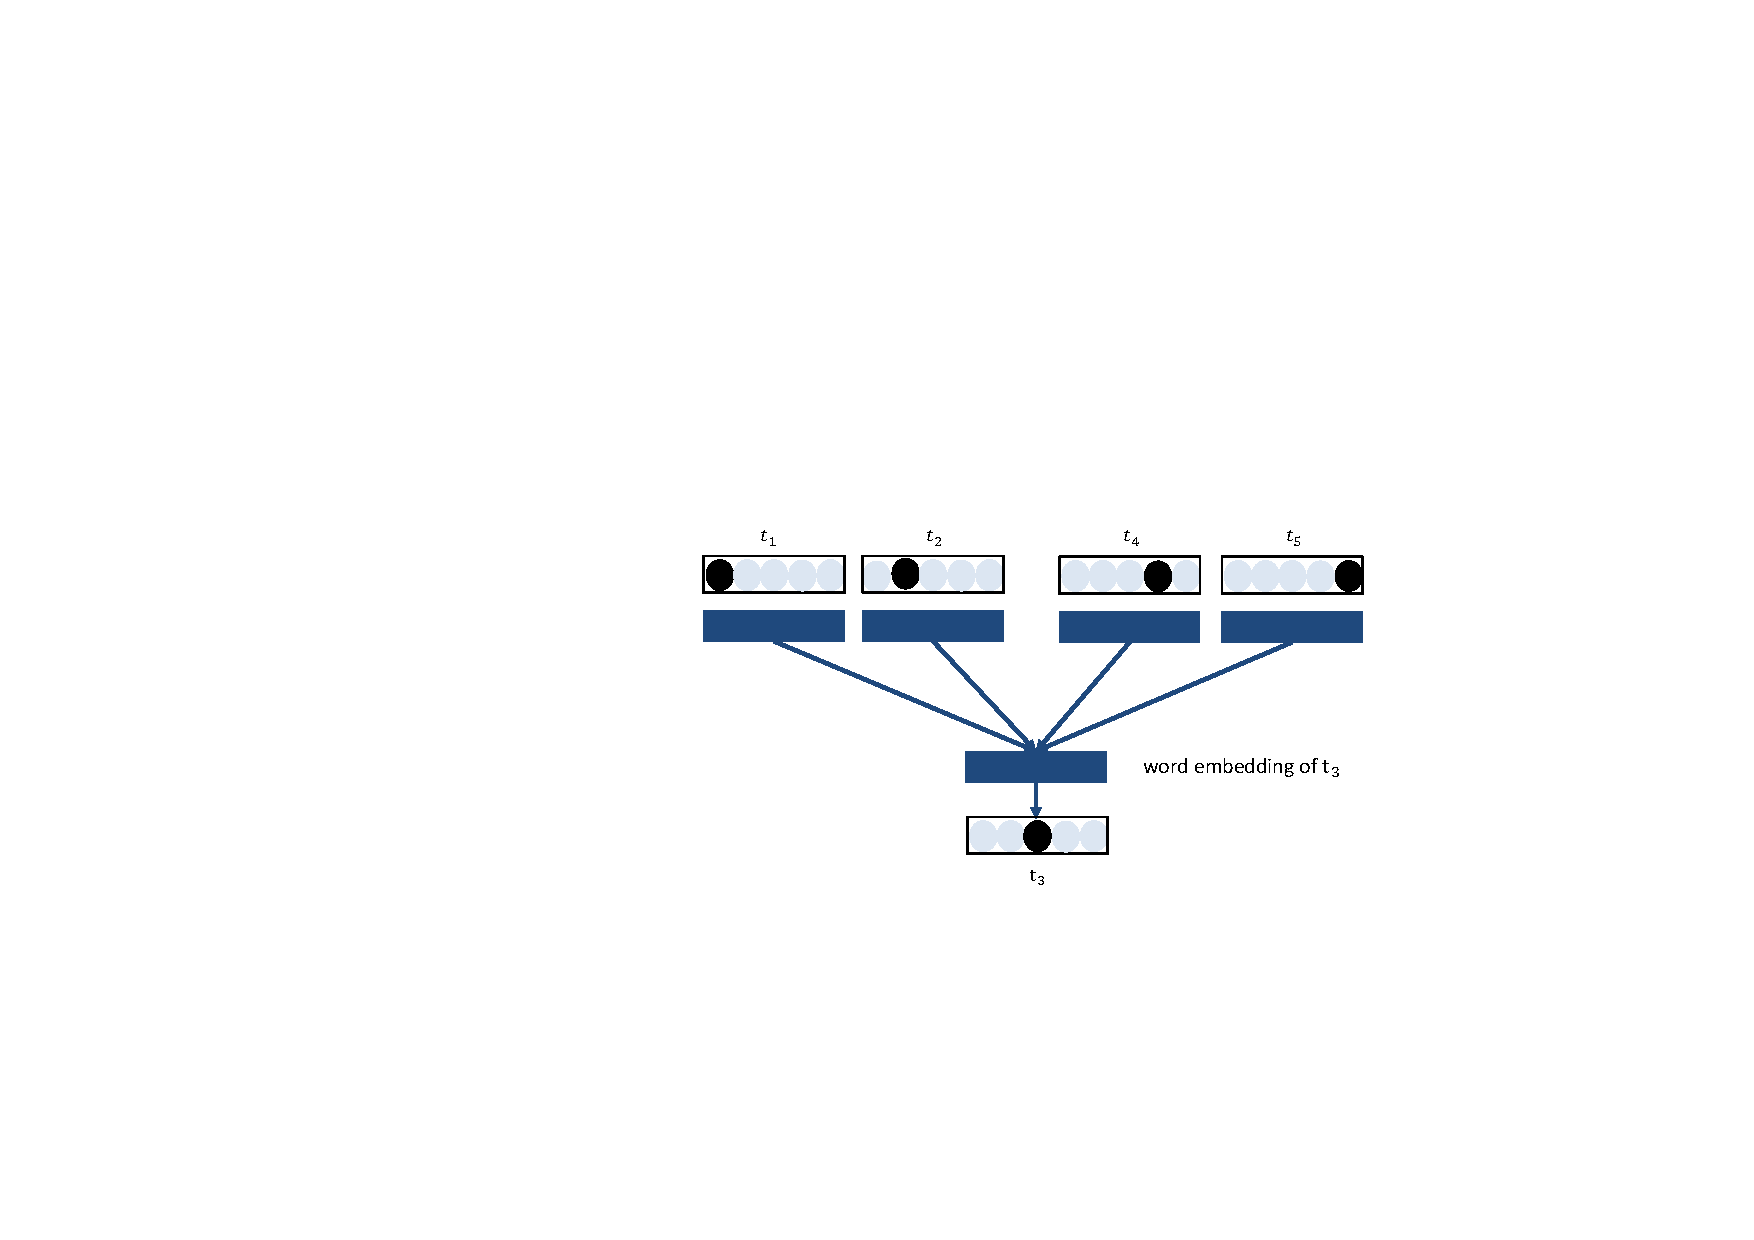
\includegraphics[width=0.23\textwidth]{figures/w2v_cbow.pdf}
		\label{fig:w2v_cbow}
	}
	\caption{The architecture of the two word embeddings models. The continuous skip-gram model predicts surrounding words given the central word, and the CBOW model predicts the central word based on the context words. Note the differences in arrow direction between the two models.
	}
	\label{fig:w2v}
\end{figure}

Word embeddings are dense low-dimensional vector representations of words that are built on the assumption that words with similar meanings tend to be present in similar context.
Studies~\cite{turian2010word, mikolov2013efficient} show that word embeddings are able to capture rich semantic and syntactic properties of words for measuring word similarity.
In our approach, given a corpus of tag sentences, we use word embedding methods to learn the word representation of each tag using the surrounding context of the tag in the corpus of tag sentences.


There are two kinds of widely-used word embedding methods~\cite{mikolov2013efficient}, the continuous skip-gram model~\cite{mikolov2013distributed} and the continuous bag-of-words (CBOW) model.
As illustrated in Fig.~\ref{fig:w2v}, the objective of the continuous skip-gram model is to learn the word representation of each word that is good at predicting the co-occurring words in the same sentence (Fig.~\ref{fig:w2v_skip}), while the CBOW is the opposite, that is, predicting the center word by the context words (Fig.~\ref{fig:w2v_cbow}).
Note that word order within the context window is not important for learning word embeddings.

Specifically, given a sequence of training text stream $t_{1}, t_{2}, ..., t_{k}$, the objective of the continuous skip-gram model is to maximize the following average log probability:
\begin{equation}
L = \frac{1}{K}\sum_{k=1}^{K} \sum_{-N\preceq j \preceq N, j\neq0} \log p(t_{k+j}|t_{k})
\label{equ:condition_skip}
\end{equation}
while the objective of the CBOW model is:
\begin{equation}
L = \frac{1}{K}\sum_{k=1}^{K} \log p(t_{k}|(t_{k-N}, t_{k-N+1}, ..., t_{k+N}) )
\label{equ:condition_cbow}
\end{equation}
where $t_{k}$ is the central word, $t_{k+j}$ is its surrounding word with the distance $j$, and $N$ indicates the context window size to be $2N+1$.
In our application of the word embedding, a tag sentence is a training text stream, and each tag is a word.
As tag sentence is short (has at most 5 tags), we set $N$ at 2 in our approach so that the context of one tag is all other tags in the current sentences.
That is, the context window contains all other tags as the surrounding words for a given tag.
Therefore, tag order does not matter in this work for learning tag embeddings.


The probability $p(t_{k+j}|t_{k})$ in Eq.~\ref{equ:condition_skip} or $p(t_{k}|(t_{k-j}, t_{k-j+1}, ..., t_{k+j}) )$ in Eq.~\ref{equ:condition_cbow} can be formulated as a log-linear softmax function which can be efficiently solved by the negative sampling method~\cite{mikolov2013distributed}.
After the iterative feed-forward and back propagation, the training process finally converges, and each tag obtains a low-dimension vector as its word representation (i.e., tag embedding) in the resulting vector space.

To determine which word-embedding model performs better in our analogical library reasoning task , we carry out a comparison experiment, and the details are discussed in Section~\ref{sec:comparison_w2v}.



\subsubsection{Mining Categorical Knowledge}

\label{sec:categoryKG}

\begin{figure}
	\centering
	\begin{tikzpicture}
	%\tikzset{level distance=1cm}
	%\tikzset{sibling distance=0.3cm}
	\tikzstyle{level 1}=[level distance=0.8cm, sibling distance=0.1cm]
	\tikzstyle{level 2}=[level distance=0.8cm, sibling distance=0.1cm]
	\tikzstyle{level 3}=[level distance=0.8cm, sibling distance=0.1cm]
	\tikzstyle{every node}=[font=\scriptsize]
	
	\Tree [.S [.NP [.NNS iOS ] ]
	[.VBZ is ]
	[.DT a ]
	[.JJ mobile ]
	[.NP [.NN operating ] [.NN system ] ]
	[.VBD developed ]
	[.IN by ]
	[.NP [.NNP Apple ] ]
	]
	
	\end{tikzpicture}
	\caption{POS tagging and phrase chunking results of the definition sentence of the tag \textit{iOS}}
	\label{fig:exampleChunking}
\end{figure}


In Fig.~\ref{fig:knowledgeGraph}, we can see that the tags can be of different categories, such as programming language, library, framework, tool, IDE, operating systems, etc.
To determine the category of a tag, we resort to the tag definition in the TagWiki of the tag.
The TagWiki of a tag is collaboratively edited by the Stack Overflow community.
Although there are no strict formatting rules in Stack Overflow, the TagWiki description usually starts with a short sentence to define the tag.
For example, the tagWiki of the tag \textit{iOS} starts with the sentence ``iOS is a mobile operating system developed by Apple''.
Typically, the first noun phrase just after the \textit{be} verb defines the category of the tag.
For example, from the tag definition of \textit{iOS}, we can learn that the category of \textit{iOS} is \textit{operating system}.
For the generality of our approach, we define \textit{noun phrase} in this work as a phrase consisting of consecutive nouns between other POS tags, including at least one noun.



Based on the above observation of tag definitions, we use the NLP methods (similar to the methods used in~\cite{kazama2007exploiting} for named entity recognition) to extract such noun phrase from the tag definition sentence as the category of a tag.
%The overview of extracting categorical knowledge can be seen in Figure.\ref{fig:flowChartCategory}.
Given the tagWiki of a tag in Stack Overflow, we extract the first sentence of the TagWiki description, and clean up the sentence by removing hyperlinks and brackets such as ``\{\}'', ``()''.
Then, we apply Part of Speech (POS) tagging and phrase chunking to the extracted sentence.
POS tagging is the process of marking up a word in a text as corresponding to a particular part of speech, such as noun, verb, adjective.
Phrase chunking is the process of segmenting a sentence into its subconstituents, such as noun phrases, verb phrases.
Different tools usually agree on the POS tags of nouns, and we find that POS tagger in NLTK~\cite{bird2006nltk}\footnote{\url{http://www.nltk.org/_modules/nltk/tag.html}} is especially suitable for our task.
In NLTK, the noun is annotated by different POS tags\footnote{\url{https://www.ling.upenn.edu/courses/Fall_2003/ling001/penn_treebank_pos.html}} including NN (Noun, singular or mass), NNS (Noun, plural), NNP (Proper noun, singular), NNPS (Proper noun, plural).
Then we use the phrase chunking i.e., regular expression to recognize consecutive nouns (at least one noun) as noun phrase by their POS tags.
%We adopt the default POS tagging and \textcolor{red}{??phrase chunking} implemented in NLTK\footnote{\url{http://www.nltk.org/_modules/nltk/tag.html}}.
%NLTK supports POS tags defined in the Penn Treebank Project\footnote{\url{https://www.ling.upenn.edu/courses/Fall_2003/ling001/penn_treebank_pos.html}}.
Fig.~\ref{fig:exampleChunking} shows the results for the tag definition sentence of \textit{iOS}.
Based on the POS tagging and phrase chunking results, we extract the first noun phrase (NP) (\textit{operating system} in this example) after the be verb (\textit{is} in this example).
We use this noun phrase as the category of the tag.
That is, the category of \textit{iOS} is \textit{operating system}.

With this method, we obtain 318 categories for the 23,658 tags (about 67\% of all the tags that have TagWiki).
We manually normalize these 318 categories labels, such as merging \textit{operating system} and \textit{os} as \textit{os}, \textit{libraries} and \textit{lib} as \textit{library}, and normalizing uppercase and lowercase (e.g., \textit{API} and \textit{api}).
As a result, we obtain 167 categories.
Furthermore, we manually categorize these 167 categories into four general categories: programming language, platform, library, and concept/standard.
These four general categories are defined in our previous work for named entity recognition~\cite{ye2016software}.
This generalization step is necessary, especially for the library tags that broadly refer to the tags whose fine-grained categories can be library, framework, api, toolkit, wrapper, and so on\footnote{A complete list can be found at \url{https://graphofknowledge.appspot.com/libCategory}}.
This is because the meaning of these fine-grained categories is often overlapping, and there is no consistent rule for the usage of these terms in the TagWiki.
For example, in Stack Overflow’s TagWiki, \textit{junit} is defined as a framework, \textit{google-visualization} is defined as an API, and \textit{wxpython} is defined as a wrapper. All these tags are referred to as library tags in our approach.


Although the above method obtains the tag category for the majority of the tags, the first sentence of the TagWiki of some tags is not formatted in the standard ``tag be noun phrase'' form.
For example, the first sentence of the TagWiki of the tag \textit{itext} is ``Library to create and manipulate PDF documents in Java'', or for \textit{markermanager}, the tag definition sentence is ``A Google Maps tool'', or for \textit{ghc-pkg}, the tag definition sentence is ``The command ghc-pkg can be used to handle GHC packages''.
As there is no \textit{be} verb in this sentence, the above NLP method cannot return a noun phrase as the tag category.
According to our observation, for most of such cases, the category of the tag is still present in the sentence, but often in many different ways.
It is very likely that the category word appears as the first noun phrase that match the existing category words in the definition sentence.
Therefore, we use a dictionary look-up method to determine the category of such tags.
Specially, we use the 167 categories obtained using the above NLP method as a dictionary to recognize the category of the tags that have not been categorized using the NLP method.
Given an uncategorized tag, we scan the first sentence of the tag's TagWiki from the beginning, and search for the first match of a category label in the sentence.
If a match is found, the tag is categorized as the matched category.
For example, the tag \textit{itext} is categorized as \textit{library} using this dictionary look-up method.
Using the dictionary look-up method, we obtain the category for 9,648 more tags.


Note that we cannot categorize some (less than 15\%) of the tags using the above NLP method and the dictionary look-up method.
This is because these tags do not have a clear tag definition sentence, for example, the TagWiki of the tag \textit{richtextbox} states that ``The RichTextBox control enables you to display or edit RTF content''.
This sentence is not a clear definition of what \textit{richtextbox} is.
Or no category match can be found in the tag definition sentence of some tags.
For example, the TagWiki of the tag \textit{carousel} states that ``A rotating display of content that can house a variety of content''.
Unfortunately, we do not have the category ``display'' in the 167 categories we collect using the NLP method.
When building analogical-libraries knowledge base, we exclude these uncategorized tags as potential candidates.

\subsubsection{Building similar-technology knowledge base}
Given a technology tag $t_1$ with its vector $vec(t_1)$, we first find most similar library $t_2$ whose vector $vec(t_2)$ is most closed to it, i.e.,
\begin{equation}
	\operatornamewithlimits{argmax}_{t_2 \in T}  \cos (vec(t_1), vec(t_2)) 
	\label{equ:similarity}
\end{equation} 
where $T$ is the set of technology tags excluding $t_1$, and $cos(u, v)$ is the cosine similarity of the two vectors.

\begin{table}
	\scriptsize
	\center	
	\begin{tabular}{l|l}
		\hline
		\textbf{Source Tech} & \textbf{Top-5 recommendations from word embedding} \\
		\hline
		nltk      & \textcolor{red}{\st{nlp}}, \textcolor{red}{\st{named-entity-recognition}}, opennlp, gate, \textcolor{red}{\st{language-model}} \\
				\hline
	\end{tabular}
	\vspace{1mm}
	\caption{Examples of filtering results by categorical knowledge (in red) \textcolor{red}{CCY: need to update with new examples}}
	\label{tab:filterResult}
\end{table}

Note that tags whose tag embedding is similar to the vector $vec(t_1)$ may not always be in the same category.
For example, tag embeddings of the tags \textit{word-sense-disambiguation}, \textit{pos-tagging} and \textit{sentiment-analysis} are similar to the vector $vec(nltk)$.
These tags are relevant to the \textit{nltk} library as they refer to some NLP concepts and tasks, but they are not analogical libraries to the \textit{nltk}.
In our approach, we rely on the category of tags (i.e., categorical knowledge) to return only tags within the same category as candidates.


In practice, there could be several similar technologies $t_2$ to the technology $t_1$.
Thus, we select tags $t_2$ with the cosine similarity in Eq.~\ref{equ:similarity} above a threshold $Thresh$.
Take the library \textit{nltk} (a NLP library in python) as an example.
We will preserve several candidates which are libraries such as \textit{textblob}, \textit{stanford-nlp}.

\subsection{Locating comparative sentences}
\textcolor{red}{Apart from Stack Overflow, we may also need to consider other related sites in Stack Exchange such as ask ubuntu, super user, unix \& linux, server fault, software engineering, software recommendation.}

\begin{table*}
	\centering
	\label{tab:pattern}
	\begin{tabular}{l l l l}
	\hline
	No. & Pattern & Sequence example & Original sentence \\ \hline \hline
	1 & \textit{TECH * VBZ * JJR} & jnnodb has 30 higher & innodb has 30 higher performance than myisam on average\\
	2 & \textit{TECH * VBZ * RBR} & post is more elegant & using post is more elegant and has more options for further development than passing them via get
\\
	3 & \textit{JJR * CIN * TECH} & slower than mysql & postgresql is slower than mysql especially when it comes to fine tuning in the end \\
	4 & \textit{RBR JJ * CIN TECH} & more powerful than velocity & freemarker is more powerful than velocity
 \\
	5 & \textit{CV * CIN TECH} & prefer ant over maven & i prefer ant over maven personally
\\
	6 & \textit{CV VBG TECH} & recommend using html5lib & i strongly recommend using html5lib instead of beautifulsoup
\\
	7 & \textit{CV TECH} & beat accurev & i have used svn cvs clearcase base ucm ccc harvest but none of them can beat accurev's strengths\\ \hline
	\end{tabular}
	\caption{The 7 comparative patterns. \textcolor{red}{CCY: 1)Please add the pattern ID at the first column. 2)For each pattern, why not consider both TECH1 and TECH2? 3)Add one column to show how many comparative sentences are extracted by this pattern. 4)replace the long examples with short sentences} }
\end{table*}

There are three steps to find comparative sentences of similar technologies.
We first carry out some preprocessing to the Stack Overflow data.
Then we locate the sentences that contain the name of any pair of similar technologies, and further spot the comparative sentences by checking if they satisfy the comparative patterns.
We will discuss these steps in detail in this section.

To extract convincing opinions about the comparison of similar technologies, we only consider answers with at least 1 score points.
Then we separate all convincing answers into individual sentences by punctuations like ``.'',  ``!'', ``?'', etc.
Note that we remove all questions sentences end with question mark, as we want to extract facts instead of doubts.
We lowercase all sentences to make them consistent with technology names because all tags are in lowercase.

\textcolor{red}{CCY: Give a table of some sample aliases}
To find sentences contain pairs of similar technologies, only using the tag names is not enough.
As posts in Stack Overflow are some informal discussion about programming-related issues, users may give different alias to the same thing.
For example, ``javascript'' can also be written in other forms such as ``js'', ``java-script'', ``javascrip'', etc.
So, aliases of software technologies are always abbreviations, synonyms, and some frequent misspellings in this work.
Such alias may lead to significant loss of comparative sentences.
Chen et al's work~\cite{chen2017unsupervised} built a large thesaurus of software-specific terms.
Based on their results, we find 7310 different alias for 3731 software technologies.
These aliases help find more potential comparative sentences.

To further identify comparative sentences from sentences containing similar technique, we propose a comparative pattern matching method. 
A sequence of POS tags is used to form a \textit{comparative pattern}. 
For example, ``\textit{RBR JJ IN}'' is a pattern that consists of a comparative adverb, a adjective and subsequently a preposition, such as "more efficient than", ``less friendly than'', etc. 
We extend the list of common POS tags to enhance the identification of comparative sentences.
More specifically, we create three comparative POS tags: \textit{CV} (comparative verbs, e.g. prefer, compare), \textit{CIN} (comparative prepositions, e.g. than, over) and \textit{TECH} (technology reference, including its name and aliases, e.g. python, eclipse).

Based on observations, we find that comparative sentences can be represented by some specific comparative patterns. 
We summarise 7 comparative patterns and corresponding examples in Table\ref{tab:pattern}.
To make the patterns more  flexible, we used a wildcard character to represent a list of arbitrary words. 
For each sentence containing similar technologies, we obtain their POS and check if any one of 7 patterns appear in them.
According to these comparative patterns, we can determine whether a sentence is a comparative sentence or not. 

\begin{comment}
The main process includes:
\begin{enumerate}
	\item Checking whether a sentence contains similar technique, including checking abbreviations and synonyms.
	\item Labeling all words in a sentence containing similar technique with common POS tags and our extended comparative POS tags;
	\item Using comparative patterns to match the sequence of POS tags. If the sentence matches at least one comparative pattern, we consider it as a comparative sentence.
\end{enumerate}}	
\end{comment}



\begin{comment}
\subsection{Extracting comparative opinions}
By analysing the sentence structure with Natural Language Processing, we extract the comparative relationships (like ``faster''), and relationship direction (like `` java --> python'').
So we transform the unstructured opinions into structured comparison. 

\subsubsection{Relationship extraction}
Observing the identified comparative sentences, we find that most of comparative relationships can be categorized into three patterns of POS tag sequence: RBR JJ (e.g. more powerful), JJR (e.g. faster) and JJR \textit{Noun} (e.g. better performance). Note that \textit{Noun} consists of NN, NNS, NNP and NNPS. We extract the part matching these three patterns in each sentence to represent the comparative relationship between the similar technique included in the sentence.
   
\subsubsection{Topic analysis}
In order to figure out what aspects of techniques users are concerned about, we conduct topic analysis based on the extracted relationships.
We use a keyword-based approach to analyze the topics. The relationships we extracted from comparative sentences are represented by ajectives (JJ), comparative adjectives (JJR) and nouns (NN, NNS, NNP and NNPS). Hence, we compile a list of keywords for each topic as Table 2 shows. The topic of each comparative sentence depends on whether this sentence contains at least one corresponding keyword.
\subsubsection{Preference Analysis} 
\end{comment}

\subsection{Extracting aspects}
After identifying comparative sentences, we extract the aspects of comparisons to summarize the comparative opinions. We utilize Word Mover's Distance to build graph for each similar technique pair and use community detection to classify comparative sentences. 
\subsubsection{Word Mover's Distance}
Word Mover's Distance (WMD) is a novel tool that allows us to accurately measure the similarity between two sentences. As Fig. ~\ref{fig:wmd} shows, the two sentences, ``\textit{postgresql} offers more security functionality than \textit{mysql}'' and "\textit{mysql} provides less safety features than \textit{postgresql}" have no words in common, but the "traveling distance" between them is small. WMD calculates the minimum amount of required distance "moving" from the embedded words of one sentence to the embedded words of another sentence~\cite{kusner2015word}. For normalization, we use WMD similarity that is simply the negative distance. For each comparative sentence, we use POS tags to extract adjectives (JJ), comparative adjectives (JJR) and nouns (NN, NNS, NNP and NNPS) as keywords to calculate WMD similarity. If the WMD similarity between comparative sentences exceeds the specified threshold, the two sentences would be added as two nodes and a linking edge to the graph for each similar technique pair. The threshold is not fixed and it depends on the difference between numbers of the extracted keywords.
\subsubsection{Community Detection}
After building graph for each similar technique pair, we use Givan-Newman algorithm to detect communities in the graph. The Givan-Newman algorithm is a hierarchical method and hence allows us to control the size of each detected community~\cite{girvan2002community}. We keep the size of communities for each similar technique pair appropriate based on the total number of comparative sentences. For each detected community, we extract the words with highest TF-IDF values as the aspect.

\begin{figure}
	\centering
	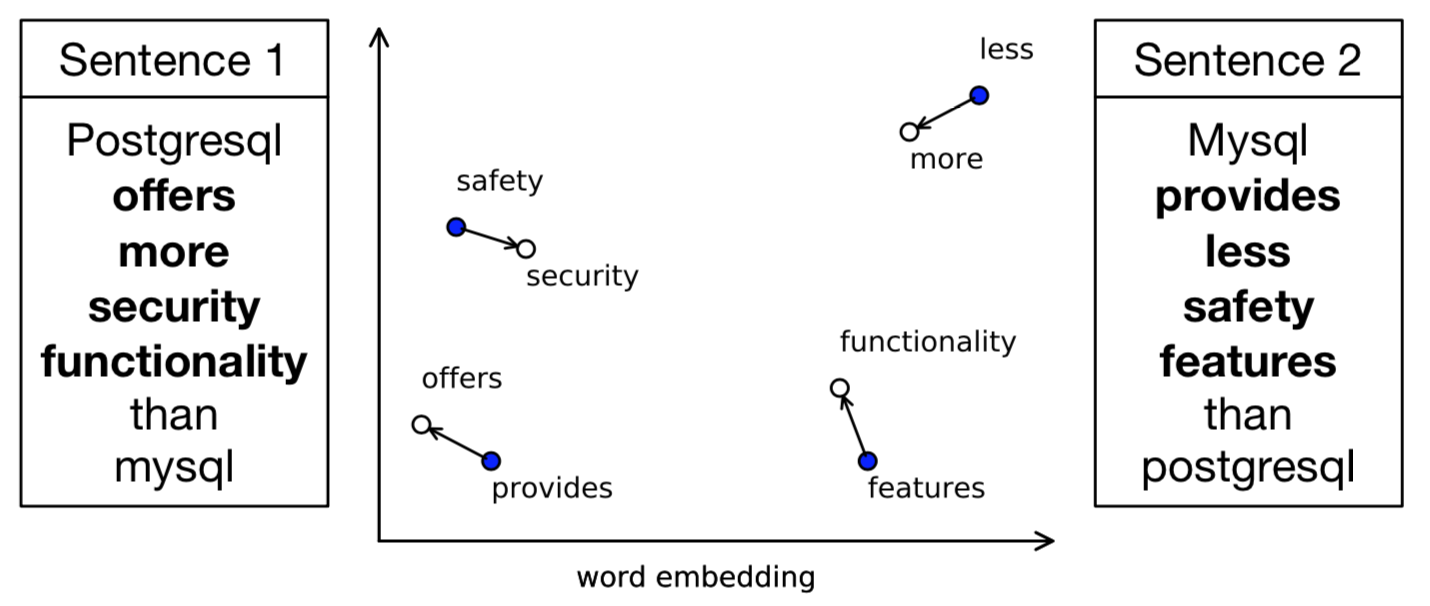
\includegraphics[width=0.5\textwidth]{figures/wmd.pdf}
	\label{fig:wmd}
	\caption{An illustration of the word mover's distance}
\end{figure}}

\subsection{Organizing the overall comparison}
We need to aggregate all individual opinions into an overview, so that users can obtain a more direct understanding of the different between the similar technique.